% Chapter 7: Neighborhoods of Universes
% Preamble-free include; colors and callout box are local conveniences.

% Local styling helpers (guarded to avoid redefinition clashes)
\makeatletter
\@ifundefined{color@deepblue}{\definecolor{deepblue}{RGB}{20, 40, 90}}{}
\@ifundefined{color@accentred}{\definecolor{accentred}{RGB}{180, 40, 40}}{}
\@ifundefined{color@boxbg}{\definecolor{boxbg}{RGB}{245, 245, 245}}{}
\@ifundefined{color@smoothgreen}{\definecolor{smoothgreen}{RGB}{34, 139, 34}}{}
\@ifundefined{color@jaggedred}{\definecolor{jaggedred}{RGB}{178, 34, 34}}{}
\@ifundefined{callout}{%
  \newtcolorbox{callout}[1]{
    colback=boxbg,
    colframe=deepblue,
    fonttitle=\bfseries,
    title=#1,
    boxrule=0.5pt,
    arc=2pt
  }
}{}
\makeatother

\chapter{Neighborhoods of Universes}
\label{chapter-7-neighborhoods-of-universes}

\section{Where alternative worlds live}

Every computation moves through \emph{time}, yes --- but that only captures the part you actually lived. The part you \emph{committed}. There is a much larger territory: the lattice of all worlds you could have entered but didn't. Reality has neighbors.

By now, you grasp the \textbf{Worldline} --- the single, irreversible trail your system carved into the causal substrate. And you've met the \textbf{Time Cone} --- the immediate shell of possible next states. But focusing only on the path behind you or the slice directly ahead is like staring through a straw at a planet. It hides nearly everything that matters.

What lives just beyond your actual decisions?\\
What universes breathe just outside your path?\\
\textit{What almost happened?}

To understand computation as geometry, you need a concept of \textbf{neighborhoods} --- the regions of Rulial Space clustering around your chosen timeline. These neighborhoods explain why certain systems feel effortless to modify, while others respond to change with the emotional maturity of a cornered raccoon.

This distinction is not academic. If you have ever tried to add a feature to a legacy codebase and felt the system push back against you --- every small change cascading into a dozen others --- you have encountered a jagged neighborhood. The system was geometrically hostile to the future you wanted. If you have ever worked in a well-designed codebase where refactors slot into place cleanly, you have experienced a smooth neighborhood. The difference is not magic. It is topology.

This chapter is about the local terrain. The lay of the land around your worldline.

Welcome to the suburbs of reality.

\begin{center}\rule{0.5\linewidth}{0.5pt}\end{center}

\section{Rules Define Locality}
\label{7.1-rules-define-locality}

Physical space uses meters. Text diff tools use lines. But the substrate of \COMPUTER{} uses neither.

The first law of locality in Rulial Space is:

\begin{quote}
\textbf{Two universes are ``near'' if you can get from one to the other using a small number of legal DPO rewrites.}
\end{quote}

This is not ``semantic closeness,'' ``visual similarity,'' or ``my gut says these states look related.'' Those are folk heuristics. Rulial geometry delivers the real metric --- and it often contradicts your intuition.

Consider two WARP graph states. One differs from your current state by a single character in a string. The other differs by a wholesale restructuring of node relationships. Which is closer? The answer depends entirely on your rewrite rules. If your rule set includes a string-editing primitive, the single-character change is one hop away. If it doesn't, that ``tiny'' change might require dismantling and reassembling entire subgraphs. Meanwhile, the ``massive'' structural change might be a single DPO application --- one legal move that transforms everything at once.

This inversion is important. It means:

\begin{itemize}
    \item A giant state difference produced by a single rewrite? $\rightarrow$ \textbf{Adjacent.}
    \item A tiny state difference requiring a labyrinth of rules to bridge? $\rightarrow$ \textbf{Distant.}
\end{itemize}

Your intuition lies; the rewrite rules don't.

And remember --- every edge in this adjacency graph may not even be a simple line. In a WARP graph, an edge can itself contain a nested graph, a whole process, a tiny universe folded into a structural tunnel. When you design your rule set, you are not just defining transitions. You are terraforming the computational cosmos. You are deciding which futures are neighbors and which are strangers.

\begin{callout}{Wormholes in WARP Graphs}
When we say ``edge,'' we don't mean a line. We mean a \textbf{tunnel}, possibly containing a full subgraph or running computation. In diagrams, it's drawn as a thin connection. In reality, it is a container. This is what makes WARP graphs recursive: the edge connecting two universes might itself be a universe.
\end{callout}

\begin{center}
    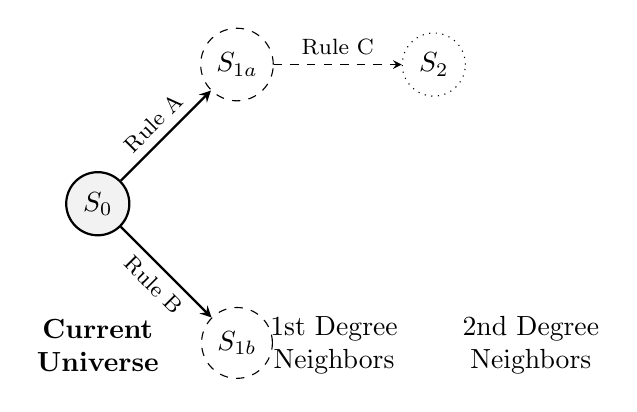
\begin{tikzpicture}[node distance=2.5cm, auto, >=stealth]
        % Nodes
        \node[circle, draw, thick, fill=gray!10] (S0) {$S_0$};
        \node[circle, draw, dashed] (S1a) [above right of=S0] {$S_{1a}$};
        \node[circle, draw, dashed] (S1b) [below right of=S0] {$S_{1b}$};
        \node[circle, draw, dotted] (S2) [right of=S1a] {$S_{2}$};
        
        % Edges
        \draw[->, thick] (S0) -- node[above, sloped, font=\footnotesize] {Rule A} (S1a);
        \draw[->, thick] (S0) -- node[below, sloped, font=\footnotesize] {Rule B} (S1b);
        \draw[->, dashed] (S1a) -- node[above, font=\footnotesize] {Rule C} (S2);
        
        % Labels
        \node[font=\bfseries, align=center] at (0,-1.8) {Current\\Universe};
        \node[align=center] at (3,-1.8) {1st Degree\\Neighbors};
        \node[align=center] at (5.5,-1.8) {2nd Degree\\Neighbors};
    \end{tikzpicture}
\end{center}

The diagram above shows the basic structure: from your current state $S_0$, applying different rules takes you to different first-degree neighbors. From those neighbors, further rules take you to second-degree neighbors. Distance in Rulial Space is measured in hops, not bytes.

\begin{center}\rule{0.5\linewidth}{0.5pt}\end{center}

\section{The Adjacency Graph of Universes}
\label{7.2-adjacency-graph}

Zoom out far enough and every possible WARP graph state becomes a node in a titanic adjacency structure. Each legal DPO rewrite becomes an edge connecting two full universes.

This is the \textbf{Graph of Universes connected by wormholes}.

Your worldline is a tiny red thread weaving through a near-infinite-dimensional combinatorial manifold. You occupy one node at a time; each clock tick pushes you along a single adjacent edge. From the inside, this feels like ``running a program.'' From the outside, it looks like a particle tracing a geodesic through state space.

Surrounding you is a shimmering halo of immediate neighbors --- worlds one rewrite away. They contain the alternative scheduler choices you did not take, the counterfactual outcomes of non-deterministic I/O (if any) baked into your model, and the shadow of every optimization you chose not to apply. These are not hypotheticals. They are real states in the adjacency graph. You could have gone there. You didn't.

Further out lie $k$-step neighborhoods: regions accessible in exactly $k$ rewrites. Their volume grows (or shrinks) with the curvature of your rule algebra. A rule set that branches aggressively will produce neighborhoods that balloon outward. A rule set with tight constraints will produce neighborhoods that expand slowly or collapse into dead-ends.

\begin{callout}{Local vs. Global}
In a high-curvature rule set, $k$-step neighborhoods can explode combinatorially or collapse into dead-ends. Neighborhood structure is therefore an empirical proxy for ``change friendliness.'' If you want to know how modifiable a system is, measure its neighborhood growth rate.
\end{callout}

The adjacency graph has another property worth noting: it is not necessarily symmetric. Just because you can reach state $B$ from state $A$ in one rewrite does not mean you can return from $B$ to $A$ in one rewrite. Some doors only open one way. This asymmetry is the geometric origin of irreversibility. When your worldline commits to a transition, it may be leaving behind states that can only be recovered through long, indirect paths --- or not at all.

\begin{center}\rule{0.5\linewidth}{0.5pt}\end{center}

\section{Smooth vs. Jagged Neighborhoods}
\label{7.3-smooth-vs-jagged}

Some systems let you hop between nearby universes with minimal effort. Others punish every deviation.

\textbf{Smooth neighborhoods} have many short rewrites connecting useful states. Refactors feel gentle. Bugs dampen out rather than cascading. Small changes stay small. The system bends when you push it. \textbf{Jagged neighborhoods} are the opposite: most short rewrites are invalid or explosive. Refactors feel brittle. Bugs cascade through the system like cracks through ice. The system shatters when you push it.

In Rulial geometry, this difference is curvature. Neighborhoods with low activation barriers are ``flat'' --- the terrain is easy to traverse in any direction. Those with cliff-like barriers are ``sharp'' --- most directions are impassable, and the few passable ones lead to dramatic drops or climbs.

This is not a metaphor. It is a measurable property of your rewrite system.

\begin{center}
    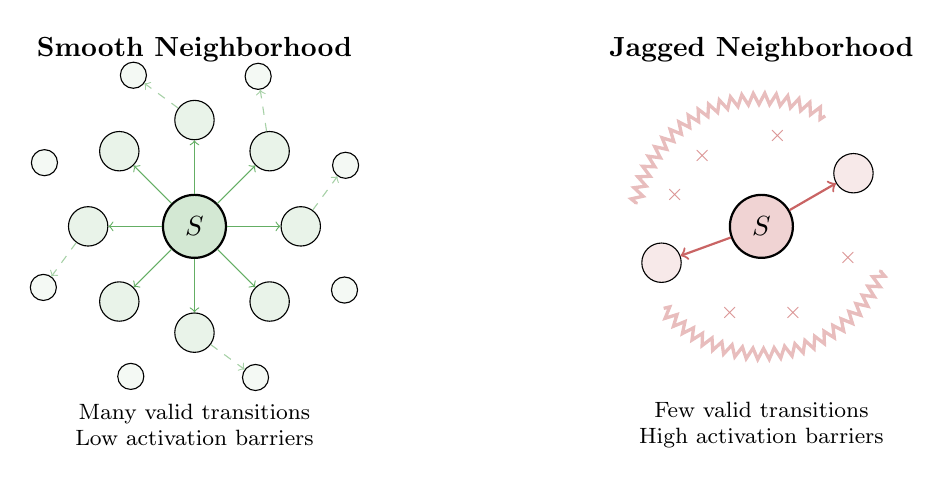
\begin{tikzpicture}[scale=0.9]
        % Smooth neighborhood (left side)
        \begin{scope}[xshift=-4cm]
            \node[font=\bfseries] at (0, 2.5) {Smooth Neighborhood};
            
            % Central node
            \node[circle, draw, thick, fill=smoothgreen!20, minimum size=0.8cm] (C1) at (0,0) {$S$};
            
            % Surrounding nodes - evenly distributed
            \foreach \i/\angle in {1/0, 2/45, 3/90, 4/135, 5/180, 6/225, 7/270, 8/315} {
                \node[circle, draw, fill=smoothgreen!10, minimum size=0.5cm] (N\i) at (\angle:1.5) {};
                \draw[->, smoothgreen!70] (C1) -- (N\i);
            }
            
            % Second ring - some connections
            \foreach \i/\angle in {1/22, 2/67, 3/112, 4/157, 5/202, 6/247, 7/292, 8/337} {
                \node[circle, draw, fill=smoothgreen!5, minimum size=0.3cm] (M\i) at (\angle:2.3) {};
            }
            \draw[->, smoothgreen!40, dashed] (N1) -- (M1);
            \draw[->, smoothgreen!40, dashed] (N2) -- (M2);
            \draw[->, smoothgreen!40, dashed] (N3) -- (M3);
            \draw[->, smoothgreen!40, dashed] (N5) -- (M5);
            \draw[->, smoothgreen!40, dashed] (N7) -- (M7);
            
            \node[font=\footnotesize, align=center] at (0, -2.8) {Many valid transitions\\Low activation barriers};
        \end{scope}
        
        % Jagged neighborhood (right side)
        \begin{scope}[xshift=4cm]
            \node[font=\bfseries] at (0, 2.5) {Jagged Neighborhood};
            
            % Central node
            \node[circle, draw, thick, fill=jaggedred!20, minimum size=0.8cm] (D1) at (0,0) {$S$};
            
            % Few valid transitions
            \node[circle, draw, fill=jaggedred!10, minimum size=0.5cm] (V1) at (30:1.5) {};
            \node[circle, draw, fill=jaggedred!10, minimum size=0.5cm] (V2) at (200:1.5) {};
            \draw[->, jaggedred!70, thick] (D1) -- (V1);
            \draw[->, jaggedred!70, thick] (D1) -- (V2);
            
            % Invalid/blocked directions shown as X marks
            \foreach \angle in {80, 130, 160, 250, 290, 340} {
                \node[font=\footnotesize, jaggedred!50] at (\angle:1.3) {$\times$};
            }
            
            % Cliff indicators
            \draw[jaggedred!30, very thick, decorate, decoration={zigzag, segment length=4pt, amplitude=2pt}] 
                (60:1.8) arc (60:170:1.8);
            \draw[jaggedred!30, very thick, decorate, decoration={zigzag, segment length=4pt, amplitude=2pt}] 
                (220:1.8) arc (220:340:1.8);
            
            \node[font=\footnotesize, align=center] at (0, -2.8) {Few valid transitions\\High activation barriers};
        \end{scope}
    \end{tikzpicture}
\end{center}

The diagram illustrates the structural difference. In a smooth neighborhood, you have many options --- eight directions, all valid, all leading to further options. In a jagged neighborhood, most directions are blocked (marked with $\times$), and the terrain itself is hostile (the zigzag boundaries represent high-energy barriers).

Why does this matter practically? Because the shape of your neighborhood determines how your system responds to change. A smooth neighborhood means you can explore alternatives cheaply. You can try different approaches, backtrack if needed, and gradually converge on a solution. A jagged neighborhood means you are trapped on narrow ridges. Every step is high-stakes. Wrong moves are expensive. The system punishes experimentation.

Most legacy codebases are jagged. Most well-designed systems are smooth. The difference is not accident. It is architecture.

\begin{center}\rule{0.5\linewidth}{0.5pt}\end{center}

\section{The Kairos Plane Expanded}
\label{7.4-kairos-plane-expanded}

The Time Cone from Chapter~\ref{chapter-5-rulial-space-rulial-distance} gave you the one-step future cone. Neighborhoods expand that picture to multiple steps and let you map gradients of effort.

Define $N_k(s)$ as the set of states reachable from $s$ in exactly $k$ rewrites. The union over all $k$ yields the future cone $F(s)$ --- everything you could ever become. But the union collapses important structure. What matters is not just \emph{where} you can go, but \emph{how far} each destination is.

Plotting the cardinality of $N_k(s)$ over $k$ is a practical way to visualize how opportunity changes with distance. The curve tells a story:

\begin{itemize}
    \item \textbf{Rapid growth of $|N_k|$}: indicates rich optionality. Good for exploration, risky for control. Your system has many degrees of freedom, and small changes can cascade into large differences. This is the signature of a creative sandbox --- or an unstable mess, depending on whether you wanted the freedom.
    
    \item \textbf{Early stagnation of $|N_k|$}: indicates constrained futures. Safe but possibly brittle. Your system converges quickly to a limited set of attractors. This is the signature of a well-constrained domain --- or a dead end, depending on whether the constraints serve you.
    
    \item \textbf{Oscillation in $|N_k|$}: indicates periodic structure in your rule algebra. Certain distances have dense neighborhoods; others are sparse. This often appears in systems with symmetry or cyclic dynamics.
\end{itemize}

The Kairos Plane is not just the immediate future. It is the complete geometry of possibility, stratified by effort. When you understand this geometry, you stop asking ``what should I do next?'' and start asking ``what does the terrain look like from here?''

\begin{center}\rule{0.5\linewidth}{0.5pt}\end{center}

\section{Navigating Neighborhoods}
\label{7.5-navigating-neighborhoods}

You can steer through neighborhoods with three levers:

\textbf{Rewrite design} shapes the topology by adding or removing rules. Every rule you introduce creates new edges in the adjacency graph. Every rule you remove destroys them. This is the most powerful lever, but also the most permanent. Once you have committed to a rule set, the geometry is largely fixed.

\textbf{Scheduler policy} biases which edges are chosen. Given the same topology, different schedulers will trace different paths. A greedy scheduler races toward local optima. A randomized scheduler explores broadly. A deterministic scheduler follows a fixed trajectory. The scheduler does not change the terrain, but it does change how you traverse it.

\textbf{State scaffolding} introduces structures that increase or dampen matchability. If you add a node that many rules can bind to, you are effectively creating a hub --- a state from which many transitions are available. If you remove such a node, you are closing off routes. Scaffolding is the middle ground between rule design and scheduling: it shapes the terrain without changing the fundamental rule set.

Navigation is not just about getting somewhere. It is about bending the local geometry so that desirable futures are closer and undesirable ones are farther. Good system design makes good outcomes easy to reach. Great system design makes bad outcomes hard to reach without making good outcomes hard to leave.

This is the deep lesson: you are not just writing code. You are sculpting the adjacency graph your code will live in. Every design decision is a choice about which futures will be neighbors.

\begin{center}\rule{0.5\linewidth}{0.5pt}\end{center}

\section{Neighborhood Pathology: When Terrain Goes Wrong}
\label{7.6-neighborhood-pathology}

Not all neighborhoods are created equal, and some are actively hostile.

\textbf{Cul-de-sacs} are states with no valid outbound transitions. Your system reaches them and stops. In a deterministic system, this is a crash or a hang. The worldline terminates.

\textbf{Tar pits} are states with valid transitions, but all of them lead back to the same region. You can move, but you cannot escape. The system churns without progressing.

\textbf{Cliffs} are states where the only valid transitions lead to dramatically different (and usually worse) neighborhoods. One wrong step, and you fall into a region where recovery is expensive or impossible.

\textbf{Mirages} are states that appear close in some naive metric (like text similarity) but are actually distant in Rulial terms. You think you can get there easily, but the actual path is labyrinthine.

Recognizing these pathologies is the first step to avoiding them. When you design a system, you are implicitly defining where these traps will appear. A well-designed system has few cul-de-sacs, no tar pits, gentle slopes instead of cliffs, and honest distances instead of mirages.

Legacy systems accumulate pathologies over time. Each quick fix, each shortcut, each ``we'll clean this up later'' adds another trap to the terrain. Eventually, the neighborhood becomes so jagged that any change is dangerous. This is technical debt, expressed geometrically.

\begin{center}\rule{0.5\linewidth}{0.5pt}\end{center}

\section*{FOR THE NERDS™}

Neighborhood analysis can be made quantitative. If you want to move from vibes to metrics, here are three tools:

\textbf{Neighborhood entropy} measures how ``spread out'' your options are at distance $k$. For a scheduler-induced probability distribution over $N_k(s)$, define:
\[
H_k(s) = -\sum_{t \in N_k(s)} p(t) \log p(t)
\]
High entropy means many roughly-equiprobable options. Low entropy means a few dominant paths. If $H_k$ drops rapidly as $k$ increases, your system funnels toward attractors. If it stays high, your system maintains optionality.

\textbf{Clustering coefficient} measures how densely interconnected $N_k(s)$ is under the rewrite graph. If neighbors of neighbors tend to also be neighbors, the clustering coefficient is high. This indicates a ``clumpy'' neighborhood structure --- states come in natural groups. Low clustering indicates a more fragmented landscape.

\textbf{Mean activation energy} is the average minimal rewrite cost to enter a basin of attraction from your current state. If different basins have different activation energies, you can map the ``effort landscape'' of your system. Low-energy basins are easy to fall into. High-energy basins require deliberate work to reach.

These measures turn intuitions into numbers. They let you compare systems, track changes over time, and diagnose pathologies before they become crises.

One more technical note: the adjacency graph we have been discussing is the \emph{state space graph} of your rewrite system. In category-theoretic terms, this is the free category generated by your rewrite rules, quotiented by any equivalences you impose. The neighborhood structure is the metric geometry induced by the categorical structure. If you find yourself wanting to prove things about neighborhoods, this is the language to use.

\begin{center}\rule{0.5\linewidth}{0.5pt}\end{center}

\section{Transition: From Neighborhoods to MRMW}
\label{7.7-transition}

We have examined the path you actually took (Worldline), the futures available at each tick (Time Cone), and the surrounding terrain (Neighborhoods). But all of this still assumes a single fixed rule set.

Think about that. Everything we have discussed --- adjacency, distance, curvature, pathologies --- depends on which rules exist. Change the rules, and the entire geometry changes. States that were adjacent become distant. Cul-de-sacs open up. Cliffs flatten into plains.

This raises a natural question: \textbf{What happens when the rules themselves change?}

How do entire rewrite models relate to one another? How do worldlines behave under different physics? How does modifying the DPO interface carve out whole new continents of computational space?

We are not just navigating a landscape anymore. We are asking about the landscape of all possible landscapes. The meta-terrain.

This is \textbf{Multi-Rewrite Multi-World (MRMW)} --- the phase space of all possible rewrite universes. Where neighborhoods give you the local structure around a single worldline, MRMW gives you the global structure across all possible rule systems.

And that is Chapter 8.